

\chapter[Proof techniques I]{Proof techniques I --- Standard methods}
\label{ch:proof1}


\section{Direct proofs of universal statements}
\label{sec:direct}

\begin{table}[hbt] 
\begin{center}
\begin{tabular}{l}
\rule{12pt}{0pt} Even \\
\framebox{\begin{minipage}{.8\textwidth}%
\rule[-6pt]{0pt}{20pt} $\forall n \in \Integers$, \\
\centerline{\rule[-6pt]{0pt}{20pt}$n$ is even \rule{6pt}{0pt} $\iff$ \rule{6pt}{0pt} $\exists  k \in \Integers, \; n = 2k$} \end{minipage} }\\
\rule{12pt}{0pt} Odd \\
\framebox{\begin{minipage}{.8\textwidth}%
\rule[-6pt]{0pt}{20pt} $\forall n \in \Integers$, \\
\centerline{\rule[-6pt]{0pt}{20pt}$n$ is odd \rule{6pt}{0pt} $\iff$ \rule{6pt}{0pt} $\exists
 k \in \Integers, \; n = 2k+1$} \end{minipage} }\\
\rule{12pt}{0pt} Divisibility\\
\framebox{\begin{minipage}{.8\textwidth}%
\rule[-6pt]{0pt}{20pt} $\forall n \in \Integers , \forall \quad d>0 \in \Integers$, \\
\centerline{\rule[-6pt]{0pt}{20pt}$d \divides n$  \rule{6pt}{0pt} $\iff$ \rule{6pt}{0pt} $\exists
 k \in \Integers, \; n = kd$} \end{minipage} } \\
\rule{12pt}{0pt} Floor\\
\framebox{\begin{minipage}{.8\textwidth}%
\rule[-6pt]{0pt}{20pt} $\forall x \in \Reals$, \\
\centerline{\rule[-6pt]{0pt}{20pt}$y = \lfloor x \rfloor$  \rule{6pt}{0pt} $\iff$ \rule{6pt}{0pt} 
$ y \in \Integers \, \; \land \, \; y \leq x < y+1$} \end{minipage} }\\
\rule{12pt}{0pt} Ceiling\\
\framebox{\begin{minipage}{.8\textwidth}%
\rule[-6pt]{0pt}{20pt} $\forall x \in \Reals$, \\
\centerline{\rule[-6pt]{0pt}{20pt}$y = \lceil x \rceil$  \rule{6pt}{0pt} $\iff$ \rule{6pt}{0pt} 
$ y \in \Integers \, \; \land \, \; y-1 < x \leq y$} \end{minipage} }\\
\rule{12pt}{0pt} Quotient-remainder theorem, Div and Mod\\
\framebox{\begin{minipage}{.8\textwidth}%
\rule[-6pt]{0pt}{20pt}$\forall n, d>0 \in \Integers$,\\
\centerline{\rule[-6pt]{0pt}{20pt}$\exists \mbox{!} q,r \in \Integers, \; n = qd + r \, \; \land \, \; 0 \leq r < d $} 
\rule[-6pt]{0pt}{20pt}\centerline{$n \; \mbox{div} \; d = q$} \newline
\rule[-6pt]{0pt}{20pt}\centerline{$n \; \mbox{mod} \; d = r$} 
\end{minipage} }\\
\rule{12pt}{0pt} Prime\\
\framebox{\begin{minipage}{.8\textwidth}%
\rule[-6pt]{0pt}{20pt}$\forall \, p \, \in \Integers$\\
\rule[-6pt]{0pt}{20pt}\centerline{$p$ is prime \rule{6pt}{0pt}%
$\iff$ \rule{60pt}{0pt} }
\rule[-6pt]{0pt}{12pt}\centerline{\rule{30pt}{0pt} $(p>1) \quad \land \quad (\forall x,y \in \Integers^+, \; p=xy \; \implies \; x=1 \, \lor \,  y=1)$} 
\end{minipage} }\\
\end{tabular}
\end{center}
\caption{The definitions of elementary number theory restated.}
\label{tab:defs}
\end{table}
\clearpage 



\noindent{\large \bf Exercises --- \thesection\ }

\begin{enumerate}
\item Every prime number greater than 3 is of one of the two forms
$6k+1$ or $6k+5$.  What statement(s) could be used as hypotheses in
proving this theorem?

\item Prove that 129 is odd.

\item Prove that the sum of two rational numbers is a rational number.

\item Prove that the sum of an odd number and an even number is odd.

\item Prove that if the sum of two integers is even, then so is their
difference.

\item Prove that for every real number $x$, $\frac{2}{3} < x < \frac{3}{4} \; \implies \; \lfloor 12x \rfloor = 8$.

\item Prove that if $x$ is an odd integer, then $x^2$ is of the form
$4k+1$ for some integer $k$.

\item Prove that for all integers $a$ and $b$, if $a$ is odd and $6 \divides (a+b)$, then $b$ is odd.

\item Prove that $\forall x\in\mathbb{R},\ x\not\in\mathbb{Z}\implies\lfloor x\rfloor+\lfloor-x\rfloor=-1$.

\item Define the \index{evenness}\emph{evenness} of an integer $n$ by:

\[ \mbox{evenness} (n) = k \; \iff \;  
 2^k \divides n \, \land \, 2^{k+1} \nmid n \]

State and prove a theorem concerning the evenness of products.


\item Suppose that $a$, $b$ and $c$ are integers such that $a \divides b$
and $b \divides c$.  Prove that $a \divides c$.

\item Suppose that $a$, $b$, $c$ and $d$ are integers with $a \neq c$.
Further, suppose that $x$ is a real number satisfying the equation

\[ \frac{ax+b}{cx+d} = 1. \]

\noindent Show that $x$ is rational.  Where is the hypothesis $a \neq c$
used?

\item Show that if two positive integers $a$ and $b$ satisfy $a \divides b$ \emph{and}
$b \divides a$ then they are equal.

\end{enumerate}


\newpage
\section{More direct proofs}
\label{sec:more}


\noindent{\large \bf Exercises --- \thesection\ }

\begin{enumerate}
\item Suppose you have a savings account which bears interest 
compounded monthly.  The July statement shows a balance of 
\$ 2104.87 and the September statement shows a balance \$ 2125.97.
What would be the balance on the (missing) August statement?
\item Recall that a quadratic equation $ax^2+bx+c=0$ has two real solutions
if and only if the discriminant $b^2-4ac$ is positive.  Prove that if 
$a$ and $c$ have different signs then the quadratic equation has two 
real solutions.
\item Prove that if $x^3-x^2$ is negative then $3x+4 < 7$.

\item Prove that for all integers $a,b,$ and $c$, if $a|b$ and $a|(b+c)$, then
$a|c$.

\item Show that if $x$ is a positive real number, then $x+\frac{1}{x} \geq 2$. 

\item Prove that for all real numbers $a,b,$ and $c$, if $ac<0$, then the quadratic
equation $ax^{2}+bx+c=0$ has two real solutions.\\
\textbf{Hint:} The quadratic equation $ax^{2}+bx+c=0$ has two
real solutions if and only if $b^{2}-4ac>0$ and $a\neq0$.

\item Show that $\binom{n}{k} \cdot \binom{k}{r} \; = \; \binom{n}{r} \cdot \binom{n-r}{k-r}$ (for all integers $r$, $k$ and $n$ with $r \leq k \leq n$). 

\item In proving the \index{product rule} \emph{product rule} in Calculus using the definition of the derivative, we might start our proof with:

\[
\frac{\mbox{d}}{\mbox{d}x} \left( f(x) \cdot g(x) \right)
\]

\[ = \lim_{h \longrightarrow 0} \frac{f(x+h) \cdot g(x+h) - f(x) \cdot g(x)}{h} \]

\noindent The last two lines of our proof should be:
\[
= \lim_{h \longrightarrow 0} \frac{f(x+h) - f(x)}{h} \cdot g(x) \; + \; f(x) \cdot \lim_{h \longrightarrow 0} \frac{g(x+h) - g(x)}{h}
\]

\[
= \frac{\mbox{d}}{\mbox{d}x}\left( f(x) \right) \cdot g(x) \; + \; f(x) \cdot \frac{\mbox{d}}{\mbox{d}x}\left( g(x) \right) 
\]

Fill in the rest of the proof.
\end{enumerate}

\newpage

\section[Contradiction and contraposition]{Indirect proofs: contradiction and contraposition}
\label{sec:contra}

\noindent{\large \bf Exercises --- \thesection\ }

\begin{enumerate}
\item Prove that if the cube of an integer is odd, then that integer is odd.

\item Prove that whenever a prime $p$ does not divide the square of an integer, 
it also doesn't divide the original integer. 
($p \nmid x^2 \; \implies \; p \nmid x$)

\item Prove (by contradiction) that there is no largest integer.

\item Prove (by contradiction) that there is no smallest positive real number.

\item Prove (by contradiction) that the sum of a rational and an irrational 
number is irrational.

\item Prove (by contraposition) that for all integers $x$ and $y$, if $x+y$ is odd, then $x\neq y$.

\item Prove (by contraposition) that for all real numbers $a$ and $b$, if $ab$ is irrational, then $a$
is irrational or $b$ is irrational.

\item A \index{Pythagorean triple}\emph{Pythagorean triple} is a set of three
natural numbers, $a$, $b$ and $c$, such that $a^2 + b^2 = c^2$.  Prove that, in a
Pythagorean triple, at least one of $a$ and $b$ is even.  Use either a proof by
contradiction or a proof by contraposition.

\item Suppose you have 2 pairs of positive real numbers whose products are 1.  That is, you have $(a,b)$ and $(c,d)$ in $\Reals^2$ satisfying $ab=cd=1$.  Prove that
$a < c$ implies that $b > d$. 
\end{enumerate}


\newpage

\section{Disproofs}
\label{sec:disproofs}


\noindent{\large \bf Exercises --- \thesection\ }

\begin{enumerate}
\item Find a polynomial that assumes only prime values for
a reasonably large range of inputs.
\item Find a counterexample to Conjecture~\ref{conj:prim} using 
only powers of 2.
\item The alternating sum of factorials provides an interesting
example of a sequence of integers.
\begin{center}
\[ 1! = 1 \]
\[ 2! - 1! = 1\]
\[ 3! - 2! + 1! = 5 \]
\[ 4! - 3! + 2! - 1! = 19 \]
et cetera
\end{center}

\noindent Are they all prime?  (After the first two 1's.)
\item It has been conjectured that whenever $p$ is prime, $2^p - 1$ is
also prime.  Find a minimal counterexample.

\item True or false:  The sum of any two irrational numbers is irrational.
Prove your answer.

\item True of false:  There are two irrational numbers whose sum is rational.
Prove your answer.

\item True or false: The product of any two irrational numbers is irrational.
Prove your answer.

\item True or false: There are two irrational numbers whose product is rational.
Prove your answer.

\item True or false:  Whenever an integer $n$ is a divisor of the square of an integer, $m^2$, it follows that $n$ is a divisor of $m$ as well.
(In symbols, $\forall n \in \Integers, \forall m \in \Integers, n \mid m^2 \; \implies \; n \mid m$.)
Prove your answer.

\item In an exercise in Section~\ref{sec:more} we proved that the quadratic 
equation $ax^2 + bx + c = 0$ has two solutions if $ac < 0$.  Find a counterexample which shows that this implication cannot be replaced with a biconditional.  

\end{enumerate}


\newpage

\section[By cases and By exhaustion]{Even more direct proofs: By cases and By exhaustion}
\label{sec:cases}


\noindent{\large \bf Exercises --- \thesection\ }

\begin{enumerate}
\item Prove that if $n$ is an odd number then $n^4 \pmod{16} = 1$.

\item Prove that every prime number other than 2 and 3 has the form
$6q+1$ or $6q+5$ for some integer $q$.  (Hint: this problem involves
thinking about cases as well as contrapositives.)

\item Show that the sum of any three consecutive integers is divisible
by 3.

\item Find the pebbling number of a graph whose nodes are the corners and 
whose edges are the, uhmm, edges of a cube.

\item A \index{vampire number}\emph{vampire number} is a $2n$ digit number $v$ that factors as $v=xy$
where $x$ and $y$ are $n$ digit numbers and the digits of $v$ are the 
union of the digits in $x$ and $y$ in some order.  The numbers $x$ and $y$
are known as the ``fangs'' of $v$.  To eliminate trivial
cases, pairs of trailing zeros are disallowed.  

Show that there are no 2-digit vampire numbers.

Show that there are seven 4-digit vampire numbers.

\item Lagrange's theorem on representation of integers as sums of squares
says that every positive integer can be expressed as the sum of at most 
4 squares.  For example, $79 = 7^2 + 5^2 + 2^2 + 1^2$.  Show (exhaustively) 
that 15 can not be represented using fewer than 4 squares.

\item Show that there are exactly 15 numbers $x$ in the range $1 \leq x \leq 100$ that can't be represented using fewer than 4 squares.

\item The \index{trichotomy property}\emph{trichotomy property} of the real 
numbers simply states that every real number is either positive or negative 
or zero.  Trichotomy can be used to prove many statements by looking at the
three cases that it guarantees.  Develop a proof (by cases) that the square of
any real number is non-negative.

\item Consider the game called ``binary determinant tic-tac-toe''\footnote{ %
This question was problem A4 in the 63rd annual %
\index{William Lowell Putnam Mathematics Competition} %
William Lowell Putnam Mathematics Competition (2002).  %
There are three collections of questions %
and answers  from previous Putnam exams available from the MAA % 
\cite{putnam1,putnam2,putnam3}% 
}
which is played by two players who alternately fill in the entries of a 
$3 \times 3$ array.  Player One goes first, placing 1's in the array and 
player Zero goes second, placing 0's.  Player One's goal is that the 
final array have determinant 1, and player Zero's goal is that the 
determinant be 0.  The determinant calculations are carried out mod 2.

Show that player Zero can always win a game of binary determinant tic-tac-toe
by the method of exhaustion.

\end{enumerate}


\newpage

\section[Existential statements]{Proofs and disproofs of existential statements}
\label{sec:exist}


\noindent{\large \bf Exercises --- \thesection\ } 

\begin{enumerate}
\item Show that there is a perfect square that is the sum of two
perfect squares.
\item Show that there is a perfect cube that is the sum of three
perfect cubes.
\item Show that the \index{well-ordering principle}WOP doesn't hold in the integers.  (This is an
existence proof, you show that there is a subset of $\Integers$
that doesn't have a smallest element.)
\item Show that the WOP doesn't hold in $\Rationals^+$.
\item In the proof of Theorem~\ref{gcd!exists} we weaseled out of
showing that $d \divides b$.  Fill in that part of the proof.
\item Give a proof of the unique existence of $q$ and $r$ in the
division algorithm. 
\item A \index{digraph}\emph{digraph} is a drawing containing a collection of points
that are connected by arrows.  The game known as \emph{scissors-paper-rock}
can be represented by a digraph that is \emph{balanced} (each point has the
same number of arrows going out as going in).  Show that there is a 
balanced digraph having 5 points.

\begin{center}
\begin{picture}(0,0)%
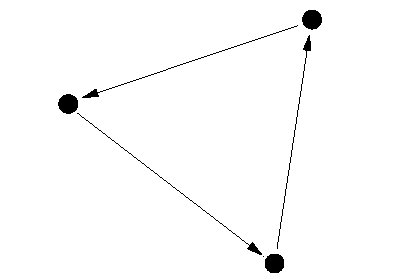
\includegraphics{./sci-pap-roc.pdf}%
\end{picture}%
\setlength{\unitlength}{3947sp}%
%
\begingroup\makeatletter\ifx\SetFigFont\undefined%
\gdef\SetFigFont#1#2#3#4#5{%
  \reset@font\fontsize{#1}{#2pt}%
  \fontfamily{#3}\fontseries{#4}\fontshape{#5}%
  \selectfont}%
\fi\endgroup%
\begin{picture}(3345,2223)(3054,-2286)
\put(5469,-1199){\makebox(0,0)[lb]{\smash{{\SetFigFont{12}{14.4}{\familydefault}{\mddefault}{\updefault}{\color[rgb]{0,0,0}smashes}%
}}}}
\put(5723,-213){\makebox(0,0)[lb]{\smash{{\SetFigFont{12}{14.4}{\familydefault}{\mddefault}{\updefault}{\color[rgb]{0,0,0}scissors}%
}}}}
\put(5381,-2271){\makebox(0,0)[lb]{\smash{{\SetFigFont{12}{14.4}{\familydefault}{\mddefault}{\updefault}{\color[rgb]{0,0,0}rock}%
}}}}
\put(3956,-1652){\makebox(0,0)[lb]{\smash{{\SetFigFont{12}{14.4}{\familydefault}{\mddefault}{\updefault}{\color[rgb]{0,0,0}covers}%
}}}}
\put(4423,-463){\makebox(0,0)[lb]{\smash{{\SetFigFont{12}{14.4}{\familydefault}{\mddefault}{\updefault}{\color[rgb]{0,0,0}cuts}%
}}}}
\put(3069,-837){\makebox(0,0)[lb]{\smash{{\SetFigFont{12}{14.4}{\familydefault}{\mddefault}{\updefault}{\color[rgb]{0,0,0}paper}%
}}}}
\end{picture}%

\end{center}
  
\end{enumerate}


%\newpage
%\renewcommand{\bibname}{References for chapter 3}
%\bibliographystyle{plain}
%\bibliography{main}

%% Emacs customization
%% 
%% Local Variables: ***
%% TeX-master: "GIAM-hw.tex" ***
%% comment-column:0 ***
%% comment-start: "%% "  ***
%% comment-end:"***" ***
%% End: ***
 
